\RequirePackage[hyphens]{url}

\documentclass[sigconf]{acmart}
\usepackage{graphicx}
\usepackage{hyperref}
\usepackage{todonotes}

\usepackage{endfloat}
\renewcommand{\efloatseparator}{\mbox{}} % no new page between figures

\usepackage{booktabs} % For formal tables

\settopmatter{printacmref=false} % Removes citation information below abstract
\renewcommand\footnotetextcopyrightpermission[1]{} % removes footnote with conference information in first column
\pagestyle{plain} % removes running headers

\newcommand{\TODO}[1]{\todo[inline]{#1}}
\begin{document}
\title{IoT and Big Data Analytics for Equipment Predictive Health Management (PHM)}
\author{Ashok Reddy Singam}
\orcid{HID337}
\affiliation{%
  \institution{Indiana University}
  \streetaddress{711 N Park Ave}
  \city{Bloomington} 
  \state{Indiana} 
  \postcode{47408}
}
\email{asingam@iu.edu}
\author{Anil Ravi}
\orcid{HID333}
\affiliation{%
  \institution{Indiana University}
  \streetaddress{711 N Park Ave}
  \city{Bloomington} 
  \state{Indiana} 
  \postcode{47408}
}
\email{anilravi@iu.edu}
\begin{abstract}
The predictive health management (PHM) is an enabling discipline consisting of technologies and methods to assess the reliability of a product in its actual life cycle conditions to determine the advent of failure and mitigate system risk. The PHM system will monitor environmental, operational, and performance related characteristics of the product and gathered data analyzed to assess product health and predict remaining life. 

In this application, the industrial rotating equipment such as compressors, vacuum blowers, pumps, and valves etc. are considered to monitor and analyze their operational behavior. The product critical operational parameter data such as vibration, temperature, and load current will be collected from field sensors and analyzed to predict the failure using kNN machine learning classification algorithms. The data will be collected from the field using wireless sensors and stored on the cloud based AWS database server. The product data will be analyzed and made available to all stake holders to take appropriate preventive actions via web/mobile applications.
\end{abstract}
\keywords{i523, HID333, HID337, KNN, IoT, Big Data, Analytics}
\maketitle
\section{Introduction}
The PHM technology can be put within a broader business context by relating it to the Product-Service System (PSS) business model. PSS can be defined as an integrated combination of products and services where the emphasis is put on the \lq sale of use \rq rather than the \lq sale of product \rq. Central to this new business model is a shift from selling a product, and its related spare parts as required, to selling a solution that supports customer needs in the form of a service delivering a fully maintained and useable product \cite{Tonci2009}. As shown in Figure \ref{F:Figure1}, There are several wireless technologies such as 802.11, cellular, and short distance wireless protocols  can be used to collect and send data to the centralized servers.Also, data can be stored in cloud based technologies such as AWS, Microsoft Azure, IBM and Google etc. for processing. 


\begin{figure}
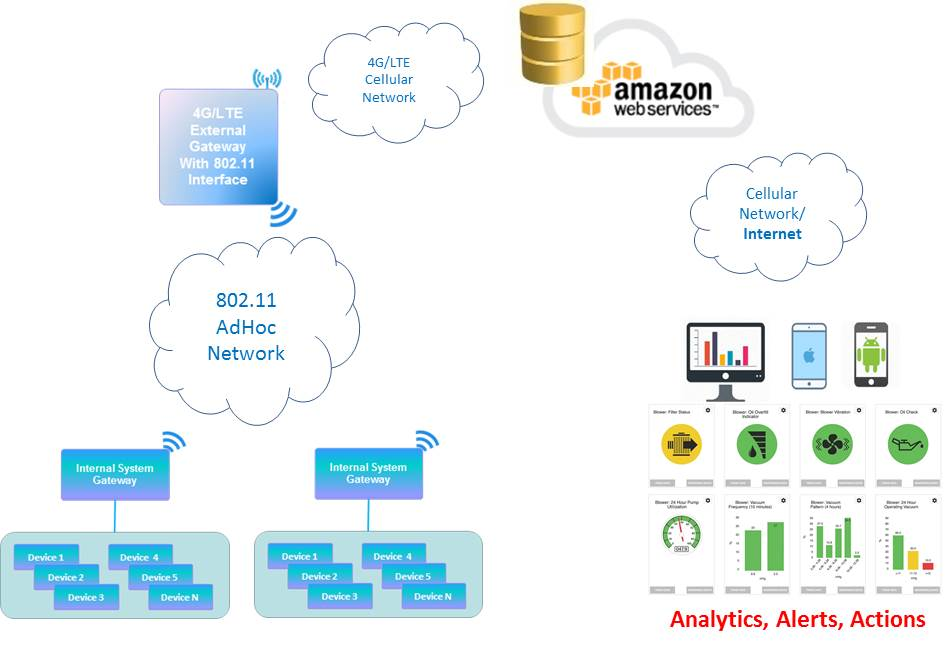
\includegraphics[width=1.0\columnwidth]{images/system_architecture}
\caption{System Architecture} \label{F:Figure1}
\end{figure}


\textbf{Problem Statement:} in the manufacturing operations, automotive and other process industries rotating equipment such as pumps, valves, compressors, and blowers are commonly used equipment for various purposes. These equipment are severely suffered from wear and tear, bearing degradation, shaft misalignment, corrosion, and other mechanical breakdowns. Due to the limitations of wireless enabled sensors based data acquisition it was very difficult to collect this data in the past. Also, due to real-time nature of the data acquisition, it was a huge challenge to store the data locally and process the information for applying machine learning algorithms. All these technological and infrastructure limitations caused industrial equipment health monitoring had become one of the sector businesses are losing the money due to operation shutdowns and unplanned maintenance etc.

\textbf{Solution Approach:} with the wireless sensors and cloud based server technologies, it has become possible to deploy hundreds of sensors in the manufacturing plant and collect the data and store with minimal costs. Once the data is stored on the servers with high computing power, machine learning algorithms can be used to process the sensor data to predict the equipment failures with reasonable accuracy. This approach has been named as predictive or prognostics health management of the equipment which is widely available in the recent times due to the availability of technological infrastructure.

The PHM generally combines sensing, collecting, storing and analyzing of environmental, operational, and performance related parameters to assess the health of a product and predict remaining useful life. Assessing the health of a product provides information that can be used to meet several critical goals \cite{Shunfeng2010}: 

\begin{itemize}
\item Providing advance warning of failures
\item Minimizing unscheduled maintenance, extending maintenance cycles, and maintaining effectiveness through timely repair actions
\item Reducing the life cycle cost of equipment by decreasing inspection costs, downtime, and inventory
\item improving qualification and assisting in the design and logistical support of fielded and future systems
\end{itemize}

The PHM is not a new concept, however, with the advent of sensors, machine learning algorithms, and computing capacity of the servers it has become more prevalent in the recent days. In this application, an attempt has been made to prove the concept of simple PHM implementation and use in real world applications. The application can be re-architected to address more complex products/systems with considerations of scalability, performance, cost and reliability. The limitations of the current application are described in the end of this report.

The parameter monitoring and the analysis of acquired data using prognostic models are fundamental steps for the PHM methods. The sensors are the essential devices used to monitor parameters and obtain long-term accurate information to provide anomaly detection, fault isolation, and rapid failure prediction \cite{Shunfeng2010}.

Firstly, PHM requires monitoring a large number of product parameters to evaluate the health of a product. Depending on the complexity of the monitored product, it is possible to monitor thousands of parameters in the entire life cycle of the product to provide the information required by PHM. These parameters include operational and environmental loads as well as the performance conditions of the product, for example, temperature, vibration, shock, pressure, acoustic levels, strain, stress, voltage, current, humidity levels, contaminant concentration, usage frequency, usage severity, usage time, power, and heat dissipation. In each case, a variety of monitoring features such as magnitude, variation, peak level, and rate of change may be required in order to obtain characteristics of parameters.

In this application, commonly used equipment in industrial and automobile operations such as air compressors, vacuum blowers, and smart valves are considered for analysis. The critical operational parameters of these products will be collected using applicable sensors from the field and fed to a database at regular intervals.

In general design, the frequency of data collection and storage depends on the number of parameters to be analyzed, cost of the system and operational behavior of the equipment. For this application, since products with rotating parts are considered, the critical parameters that would define the health of the equipment are: input or load current, internal ambient temperature, and vibration of the equipment.

The PHM application design process is shown in Figure \ref{F:Figure2}, which describes various steps of the processes involved. For the implementation of this project, the sensor generated data is simulated using SQL scripts due to development time constraints. However, a detailed step-by-step approach is provided if we need to plug-in the sensor modules in to the application.



\begin{figure}
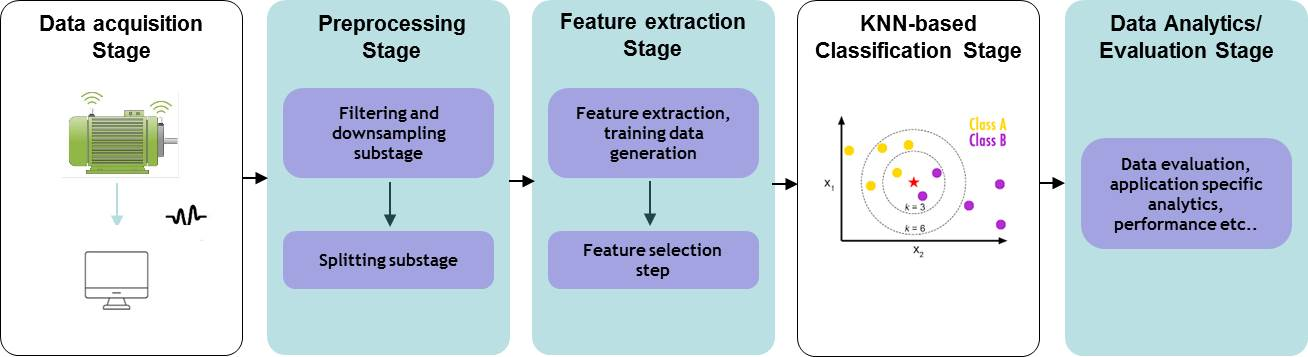
\includegraphics[width=1.0\columnwidth]{images/phm_process_1}
\caption{PHM Design Process} \label{F:Figure2}
\end{figure}



\textbf{Data Acquisition Stage:} It is required to have a description of a machine behaving normally that can be used for
early detection of anomalies. This calls for a proper characterization of machine health. As part of this process, various methods are identified to extract health information from vibration measurements and investigate strengths and weaknesses of these methods as health descriptors. This stage will be the core part of PHM application where vibration data were experimentally obtained from a compressor using triaxial accelerometer to collect transverse, longitudinal and vertical axes vibration signals. For the experimental data collection, ACC301A triaxial accelerometer and National Instruments data acquisition system was used. A total of 8 parameters 
\begin{enumerate}
\item Input Current
\item Input Voltage
\item Internal ambient temperature
\item External ambient temperature
\item Transverse vibration
\item Longitudinal vibration 
\item Vertical axis vibration
\item Acquisition time
\end{enumerate}
were captured at one second rate, which generated about 65000 records. This data has been analyzed for identifying the feature classification.

\textbf{Pre Processing stage:} During this stage collected data will be filtered and processed for accuracy in order to adapt them to subsequent feature extraction stage. In this application, all the pre-processing has been done manually to validate the accuracy of the data based on the system conditions. Since spectral analysis of vibration signals are not done ( one of the limitations for this application, captured in the end), the data generated from the compressor is considered as the primary frequency of the equipment (which is isolated from the rest of the attachments).

\textbf{Feature extraction and selection stage:} during this stage domain specific vibration spectral analysis has been performed but only considered time-domain behavior for various system operational conditions such as increased load, modified input voltage, and modified external ambient temperature etc. Based on the response of the machine vibration to various external conditions were noted down. This data is used to identify the following feature vectors.
\begin{itemize}
\item NORMAL OPERATION AT 30 DEG CENTIGRADE
\item OVER CURRENT FAULT OPERATION
\item OVER TEMPERATURE FAULT OPERATION
\item INPUT OVER VOLTAGE FAULT OPERATION
\item ABNORMAL OPERATION AT 30 DEG CENTIGRADE
\item BEARING DEGRADATION OPERATION
\end{itemize}


\textbf{kNN classification stage:} this stage is core part of the PHM application, which will predict the unknown test data to be classified in to a known label based on the training data set using nearest neighbor algorithm.

\textbf{Classifier performance evaluation stage:} this stage will be used to evaluate the classifier accuracy of prediction. In this application, k-fold cross-validation method has been used to perform the evaluation.

The data is generated and made available in Oracle database on AWS cloud to perform analysis. The application developed in this project will consist of the following components:
\begin{itemize}
  \item Sensor Data Generator
  \item Machine Learning Algorithm
  \item Big Data and IoT
  \item PHM Dashboard
  \item Decision Alerts
  \item Application Script
 \end{itemize}

The following sections will describe the architectural and design aspects of the PHM system implementation in detail.

\section{Prognostics Model Evaluation}
\cite{Saxena2009} The prediction is typically performed only after the \textit{health} of the component or system deteriorates beyond a certain threshold. In this application, faults and failures are identified in the training data set. The faults identified are: Over current fault, over temperature fault and over voltage fault. If over current fault is occurred, the equipment will tend to draw higher current than nominal values which if continued further several times eventually leads to a permanent failure of the equipment. In this application, when motor bearing starts degrading, the first observation will be over current followed by over temperature conditions.
Often times, that threshold is tripped because a fault occurs. A fault is a state of a component or system that deviates from the normal state such that the integrity of the component is outside of its required specification. A fault does not necessarily imply that the overall system does not operate anymore; however, the damage that characterizes the fault often grows under the influence of operations to a failure. The latter is the state at which the component or system does not meet its desired function anymore. It is the task of prognostics to estimate the time that it takes from the current time to the failed state, conditional on anticipated future usage. This would give operators access to information that has significant implications on system safety or cost of operations. Where safety is impacted, the ability to predict failure allows operators to take action that preserves the assets either through rescue operation or through remedial action that avert failure altogether. Where minimizing cost of operations is the primary objective, predictive information allows operators to avert secondary damage, or to perform maintenance in the most cost-effective fashion. Often times, there is a mix of objectives that need to be optimized together, sometimes weighted by different preferences.

As emphasized above, predictive models evaluation needs to take domain specificities into account. Such specificities cover two aspects: capability of failure prediction and TTF estimation. From the point of view of TTF, it is desirable that a predictive model can generate alerts in a \textit{targeted} time window prior to a failure. A model that predicts a failure too early leads to non-optimal component use \cite{Yang2014} which will impact the reliability or availability of the system.

\begin{figure}
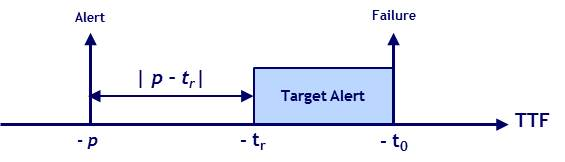
\includegraphics[width=1.0\columnwidth]{images/ttf_1}
\caption{Time relation between alert time and failure time} \label{F:Figure3}
\end{figure}

As shown in the Figure \ref{F:Figure3}, the time to failure prediction will be estimated based on the classified result data set and alert the stakeholders to take relevant actions. The target alert zone will be identified based on the abnormal behavior of the equipment over the period.

\section{Application Design Analysis}
The PHM application in this project considered to use rotating equipment temperature, load current and vibration data for analyzing and predicting the future operational behavior. 
Vibration signals from rotating components are usually analyzed in the frequency domain, because significant peaks in the signal spectrum appear at frequencies that are related to the rotation frequency of the component. In this application, only time domain parameters with peak vibration magnitudes irrespective of the frequency component. The training data set consists of normal, abnormal, and fault conditions vibration patterns describes the system characteristics from which its status can be estimated.
The PHM application for industrial equipment machine failure detection problem directly correlates to the pattern classification problem. From the vibration data collected, each accelerometer will output values of X, Y, and Z data then using a KNN we can similarly identify which vibration parameter(s) determines problems in our machines, or \textit{likely to experience failure.} The typical defects or failures that can be detected are: machine imbalance, shaft misalignment, pumps cavitation, structural and rotating looseness, early stage bearing wear, gear teeth problems, and other high-frequency defects.

This application used \textit{Sensor Data Gen} SQL script module to generate the sensor data and store in Oracle database on AWS. This is the critical module as we have not used the real data collection from the field. However, the sensor hardware and necessary environment to generate the data is identified and experimented to work with. A brief description about the hardware is provided in the end of this report.

The PHM application is designed such that the fundamental concepts can be verified to open a discussion on limitations, performance, scalability, ROI and reliability of the system.

The following sections describe the application design components with necessary implementation details:
\subsection{Sensor Data Generator}
The SQL data generator script is designed to generate training data as well test data for this application with following eleven parameters: Acquisition time, equipment name, part number, serial number, internal ambient temperature, external ambient temperature, input voltage, input current, and vibration data for x, y, and z axes. 
The following database design architecture followed for Sensor Data Gen module:
\begin{itemize}
  \item Sensor Data Generator PL SQL Objects
  \begin{itemize}
  \item Tables
\begin{itemize}
\item SENSOR TRAIN DATA for storing training data
\item SENSOR TEST DATA for storing testing data
\end{itemize}
\item Views
\begin{itemize}
\item SENSOR TRAIN DATA VIEW:
      Created View on top of SENSOR TRAIN DATA with logic to translate string label data into numbers
\item SENSOR TEST DATA VIEW
      Created View on top of SENSOR TEST DATA with logic to translate string label data into numbers
\end{itemize}
\item Packages BIG DATA 503 PRJ PKG
\begin{itemize}
\item Generate Test Set:
      Pl/Sql procedure to insert sensor test data into SENSOR TRAIN DATA table
\item Generate Train Set:
      Pl/Sql procedure to insert sensor train data into SENSOR TRAIN DATA table
\item Delete Data Set:
      Pl/Sql procedure to delete all training and test data.
\item Update Test Data Labels:
      Pl/Sql procedure to update SENSOR TRAIN DATA table with KNN algorithm predicted label values
\end{itemize}
\end{itemize}
\end{itemize}

\subsection{Machine Learning Algorithm}
\subsubsection{Classifier evaluation}
Typical classifier evaluation methods include ROC Curves, Reject Curves,Precision-Recall Curves, and Statistical Tests. The statistical tests consists of following methods to perform evaluation:
\begin{itemize}
    \item Estimating the error rate of a classifier
    \item Comparing two classifiers
    \item Estimating the error rate of a learning algorithm
    \item Comparing two algorithms
\end{itemize}

Out of the listed statistical tests, the error rate estimation method is used in this application to evaluate the performance. An experimental data is used to estimate the error rate or accuracy of various classifiers. Then a comparison has been made to choose the classifier to use in the application.

The following list of performance for various classifiers is observed during the accuracy calculation. The same set of training data has been used for all the classifiers, which has resulted the following performance. All values are mentioned in percents between 0 to 1, 1 means 100 percent accuracy.
\begin{itemize}
\item LogisticRregression: 0.963636 
\item KNN: 0.981818 
\item DecisionTreeClassifier: 0.964394 
\item SVM: 0.972727 
\end{itemize}

Based on the performance as shown in Figure \ref{F:Figure4}, kNN has been selected to use for this application. 

\begin{figure}
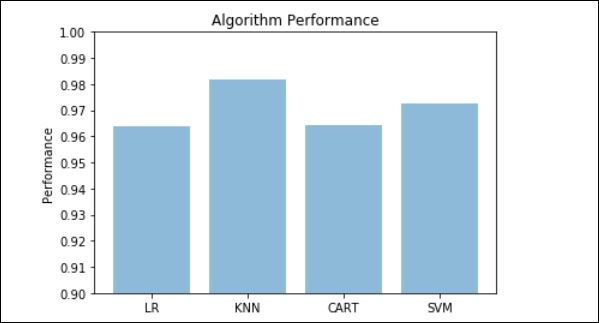
\includegraphics[width=1.0\columnwidth]{images/algperformance}
\caption{Algorithm performance} \label{F:Figure4}
\end{figure}

\subsubsection{k Nearest Neighbor - kNN}
\cite{Kevin2016} In this application, neighbors-based classification is chosen to classify the unknown instance to the known trained labels. Neighbors-based classification does not attempt to construct a general internal model, but simply stores instances of the training data.


Classification is computed from a simple majority vote of the nearest neighbors of each point: a query point is assigned the data class which has the most representatives within the nearest neighbors of the point.


KNN falls in the supervised learning family of algorithms. Informally, this means that we are given a labelled dataset consisting of training observations (x,y) and would like to capture the relationship between x and y. More formally, our goal is to learn a function \[h:X ->Y\] so that given an unseen observations x, h(x) can confidently predict the corresponding output y.


In the classification setting, the K-nearest neighbor algorithm essentially boils down to forming a majority vote between the K most similar instances to a given unseen observation.
The number of neighbors for k-nearest neighbors (k) can be any value less than the number of rows from dataset. Looking at only a few neighbors makes the algorithm perform better but the less similar the neighbors, the worse the prediction will be. Similarity is defined according to a distance metric between two data points. A popular choice is the Euclidean distance given by:


\[
d(x,x')=\sqrt{(x1-x1\rq)^2+(x2-x2\rq)^2+...+(xn-xn\rq)^2}
\]


But other measures can be more suitable for a given setting and include the Manhattan, Chebyshev and Hamming distance. 
An alternate way of understanding KNN is by thinking about it as calculating a decision boundary (i.e. boundaries for more than 2 classes) which is then used to classify new points.

Another characteristic of KNN is it is instance based learning algorithm. Means it doesn't explicitly learn a model. Instead, it chooses to memorize the training instances which are subsequently used as knowledge for the prediction phase.  It is also means the algorithm does not build a model until the time that a prediction is required. It is also lazy learning because it only does work at the last second. This has the benefit of only including data relevant to the unseen data, called a localized model. A disadvantage with lazy model is it can be computationally expensive to repeat the same or similar searches over larger training datasets. 

In the application design, sci-kit open source python libraries are used for implementing the kNN algorithms. Scikit is built on NumPy, SciPy, and matplotlib. The k-neighbors classification in KNeighborsClassifier is the more commonly used of the two techniques. The optimal choice of the value k is highly data-dependent: in general a larger k suppresses the effects of noise, but makes the classification boundaries less distinct.

The sklearn.neighbors.KNeighborsClassifier class has the following methods, which are used in the application design:

\begin{itemize}
\item fit: Fit the model using X as training data and y as target values.
\item get params: Fit the model using X as training data and y as target values.
\item kneighbors: Finds the K-neighbors of a point.
\item kneighbors graph: Computes the (weighted) graph of k-Neighbors for points in X.
\item predict: Predict the class labels for the provided data.
\item predict proba: Return probability estimates for the test data X.
\item score: Returns the mean accuracy on the given test data and labels.
\item set params: Set the parameters of this estimator.
\end{itemize}

\subsubsection{K-fold cross-validation}
To estimate the test error in the model, a cross-validation approach followed in which a subset of the training set will be holding out from the fitting process. This subset, called the validation set, can be used to select the appropriate level of flexibility of our algorithm. There are different validation approaches that are used in practice, and we will be exploring one of the more popular ones called \textbf{k-fold cross validation.}
The k-fold cross validation (the k is totally unrelated to K) involves randomly dividing the training set into k groups, or folds, of approximately equal size. The first fold is treated as a validation set, and the method is fit on the remaining \(k-1\) folds. The misclassification rate is then computed on the observations in the held-out fold. This procedure is repeated k times; each time, a different group of observations is treated as a validation set. This process results in k estimates of the test error which are then averaged out. 

In this application, an average k-fold cross validation accuracy of 0.99 percent achieved, which is explained in the appendix section of the report. Figure \ref{F:Figure8} shows Classification and Confusion report output obtained from the KNN model we used for this project.

\begin{figure}
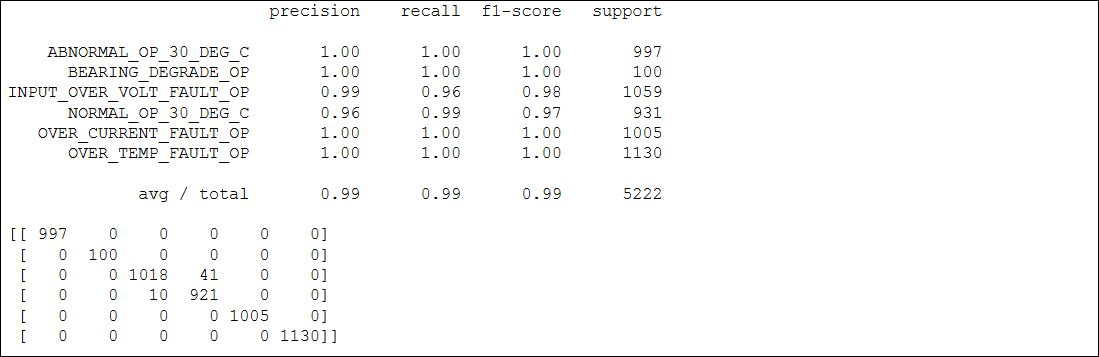
\includegraphics[width=1.0\columnwidth]{images/knnclassification}
\caption{KNN Classification and Confusion matrix report} \label{F:Figure8}
\end{figure}

\subsection{Big Data and IoT}
In PHM systems big data is characterized by one or more 3Vs: volume, velocity and variety due to streaming of real-time IoT sensors. Most of the IoT systems present challenges in combinations of velocity and volume. The important feature of the IoT application is that by observing the behavior of \lq\lq many things\rq\rq it will be possible to gain important insights, optimize processes, etc. This requires storing all the events (velocity and volume challenge) to run analytical queries over the stored events and perform analytics (data mining and machine learning) over the data to gain insights.
In general PHM applications, data will be collected through field sensors at specific rate which accounts for large amount of data per day in the order of multi-million records. This data will be stored in any NOSQL or RDBMS based database for storage and processing. Since the big data infrastructure is much reliable and available widely from multiple vendors, it would help to build complex PHM systems with large number of feature vectors for classification. 

In this application, for the demonstration of the concept, the real vibration data from the compressor equipment has been collected via accelerometer sensors. This vibration data has been analyzed in time domain and established the labels based on the compressor design performance parameters. Later, this data analysis is used to design a SQL script for generating training and test data sets. However, the real-time PHM system will have continuous streaming of data coming from hundreds of devices at faster rates (in the order of milliseconds to tens of seconds). This data needs to be captured by reliable and scalable platforms such as AWS IoT or similar and use the machine learning algorithms to classify the unknown data.
\subsection{PHM Dashboard}
Once all the test data set has been classified in to appropriate labels, the prediction of the failure can be performed based on the trending of the equipment behavior over the period. In order to understand the equipment performance insight, following queries will be used on the classified data:
\begin{itemize}
  \item Faults Reported by Equipment Part Number
  \item Faults Reported by Serial Number
  \item Abnormal Behavior by Equipment Part Number
  \item Abnormal Behavior by Serial Number over the period range
\end{itemize}
There can be more application specific information obtained from classified data set to take various decisions. Figure \ref{F:Figure5}, Figure \ref{F:Figure6} and Figure \ref{F:Figure7} show various PHM data analytics for this project. Figure \ref{F:Figure5} displays all the serial numbers of equipment 1 with bearing degradation problems. The X axis gives serial numbers while the Y axis gives number of occurrences of bearing degradation for that particular serial number. Similarly Figure \ref{F:Figure6} and Figure \ref{F:Figure7} give the details of over temperature and over current faults of various serial numbers.

As part of data visualization, result data file is queried based on the analytics metrics interested. The python matplotlib package has been used to draw the charts as needed for showing the analytics. In real world application, a more sophisticated business intelligence tools such as Tableau, Microsoft BI, and Amazon Quick Sight can be used to show the PHM dashboards. These dashboards are targeted for business users so that they will be able to customize the views, add filters and drill down in to specific information as needed. 

Sample screen shots for the following scenarios are included from python code output:

\begin{itemize}
  \item Bearing Degraded Serial numbers for Equipment Part Number1: Figure \ref{F:Figure5}
  \item Over Temperature Fault Serial numbers for Equipment Part Number1: Figure \ref{F:Figure6}
  \item Over Current Fault Serial numbers for Equipment Part Number1: Figure \ref{F:Figure7}
\end{itemize}

\begin{figure}
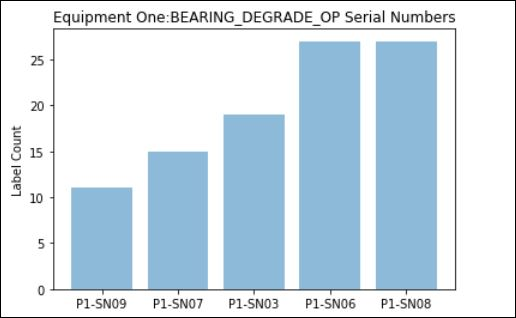
\includegraphics[width=1.0\columnwidth]{images/DEGRADE}
\caption{Bearing Degradation} \label{F:Figure5}
\end{figure}

\begin{figure}
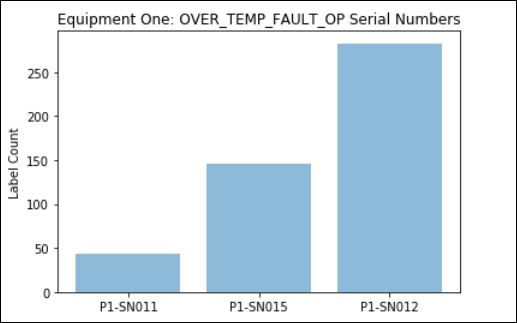
\includegraphics[width=1.0\columnwidth]{images/OVERTEMP}
\caption{Over Temperature Fault} \label{F:Figure6}
\end{figure}

\begin{figure}
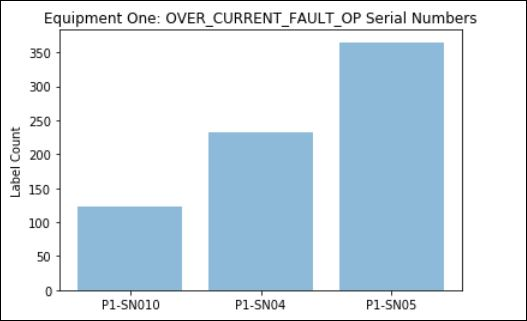
\includegraphics[width=1.0\columnwidth]{images/OVERCURR}
\caption{Over current Fault} \label{F:Figure7}
\end{figure}

\subsection{Decision Alerts}
Once the results data set has been generated by the prediction algorithm, and then based on the analytics queries, PHM system can send out the alert messages to appropriate stakeholders. The typical messages include the following s minimum:
\begin{itemize}
  \item SN 10002: Faulted X times on over temperature in last Y days, needs maintenance to clean the filter
  \item SN 10005: Consistently indicating bearing degradation from last X days, needs lubrication maintenance
\item SN 10009: Consistently drawing over current from last X days, needs mechanical load maintenance
\end{itemize}

In this application all the unseen test data is classified and labeled in the result data file. However, in real world application, along with the dashboards a comprehensive alerting capabilities can be built. The application checks for out of range alert conditions on selected incoming report parameters, looking for warning or alarm conditions that are higher or lower than expected under normal operating conditions.

\subsection{Application Code Development}
Code required for this project is divided into two categories
\begin{itemize}
    \item Python Coding:
          We used \textbf{Anacoda Navigator ver 1.6.9} \cite{Anaconda2017} installation on windows7 laptop which includes Jupyter notebook application for python coding. \textbf{Anacoda Navigator} also supports multiple installation and management of python environments using gui interface. The location of the Jypyter notebook file we developer for this project is mentioned in appendix b.
    \item Pl/SQL Coding:
          This application specific training/test sensor data has been created/generated on AWS cloud database using pl/sql coding which will be accessed during the run time by python notebook. We used \textbf{Orcle Sql Developer } \cite{SQLDeveloper2017} for pl/sql coding.
\end{itemize}
\subsection{Python - Oracle Interface}
For this project we used python library called \textbf{cxOracle} \cite{OracleOTN} to enable access to Oracle Database. It can be installed easily using \textbf{pip} and it supports both Python 2 and 3. This library supports:
\begin{itemize}
  \item SQL and PL/SQL Execution. The underlying Oracle Client libraries have significant optimizations including compressed fetch, pre-fetching, client and server result set caching, and statement caching with auto-tuning.
  \item Extensive Oracle data type support, including large object support like CLOB and BLOB)
  \item Batch operations for efficient INSERT and UPDATEs
\end{itemize}

In the following scenarios we used \textbf{cxOracle} libraries:

\begin{itemize}
  \item To read sensor training data from Oracle database
  \item To read sensor test data from Oracle database
  \item After classification of labels, to update test data with classified labels
\end{itemize}

\section{Application Limitations}
The PHM application developed in this project has several limitations. Typically, PHM applications suffer from the prediction accuracy rate which influences the ability to take decisions that will have broader impact on the business operations and financial aspects. However, with the advanced machine learning classifiers and model evaluation methods this can be addressed to achieve reasonable confidence. Following are some of the limitations of this application, which can be addressed and improved in large real-time PHM systems.

\textbf{Data acquisition hardware:} in this application the data is not collected from real-time sensors for voltage, current, temperature and vibration data. There will be inherent accuracy in the raw data generated by SQL script. However, a sample vibration dataset has been collected from the field, which is used as basis to generate the simulated data set.

\textbf{Feature extraction analysis:} the equipment performance parameters of interest need to be down selected from large set of incoming parameter data. 


When analyzing vibration data in the time domain only few parameters are available in quantifying the strength of a vibration profile: amplitude, peak-to-peak value, and RMS.  
The amplitude is valuable for shock events but it does not take into account the time duration and thus the energy in the event. The same is true for peak-to-peak with the added benefit of providing the maximum excursion of the wave, useful when looking at displacement information, specifically clearances. The RMS value is generally the most useful because it is directly related to the energy content of the vibration profile and thus the destructive capability of the vibration.


This requires in-depth domain specific analysis, in this case a detailed mathematical modeling of vibration spectral analysis to precisely select the features and corresponding behavior patterns. Such analytical data should be used for training data feature set. In this application, a primitive approach of time-domain analysis of vibration magnitudes used for determining features. However, in real application these features need to be mathematically analyzed to identify the features that represent the system behavior as close as possible.

\textbf{Model accuracy and scoring :} the kNN algorithm used in this application validated using k-cross fold cross-validation. There are several other model evaluation and scoring methods such as accuracy (or error rate), True Positive Rate (TPR), False Positive Rate (FPR), False Negative Rate (FNR), True Negative Rate (TNR), sensitivity etc. These metrics provide a simple and effective way to measure the performance of a classifier. This application can be further improved by applying more performance measurement methods to increase the effectiveness of the algorithm design.   

\textbf{Scalability:} the application designed in this project is very primitive to understand the basic concepts of PHM and kNN classifier implementation. This application cannot be used for PHM application in business use. To implement real world PHM application, a more comprehensive design needed by considering modularity, service oriented architecture, large number of sensors integration, big data and analytics integration etc.

\section{Recommendations}
\textbf{Generality:} since each rotating equipment vibrates in a different manner, a monitoring method needs to be retrained for each machine. The training on several repeated measurements on several similar equipment in several operating modes may allow for a more general monitoring method.

\textbf{Feature extraction and dimensionality:} In this application it has been assumed that a proper feature (selection) has been chosen, such that the feature dimensionality is not too high. If the data lies in a subspace, application of an initial dimensionality reduction may be a good idea. It is highly recommended to perform spectral analysis on vibration data and identify various fault frequencies and their sources. This would help to extract the optimized feature vectors for the given application followed by selecting the more relevant ones. 

\textbf{Model evaluation:} classifier accuracy and effectiveness will be varied based on the test data set. It is highly recommended to evaluate multiple models with appropriate test data to choose the best classifier for the given application.

\textbf{Domain specific modeling:} It is highly recommended to perform more and more domain-oriented feature vector analysis to meet the needs of predictive model evaluation for PHM applications. Domain-oriented approaches helpful and useful in evaluating classifier for applications. Generic evaluation methods could help developers in investigating overall performance of a model from the statistical viewpoint at the initial stage of model development. Domain-oriented approaches should be further used to evaluate the usefulness and business value \cite{Yang2014}.  

\section{Conclusion}
In this project, the problem statement around industrial rotating equipment maintenance is described and solution principle to address the same using PHM concept is defined, experimented and results are discussed. Since this application is developed to prove the only concept but not the complete solution a section with limitations and recommendations for real world system development is described. Overall, PHM application with kNN classifier algorithm and cross validation accuracy of 0.99 percent has been implemented, verified and results are analyzed for business decisions.


\bibliographystyle{ACM-Reference-Format}
\bibliography{report} 
\newpage
\appendix
\section{Work Breakdown}
\subsection{HID 333:Anil Ravi}
\begin{itemize}
  \item Identified Project topic.
  \item Created architecture of the application.
  \item Ran experimental test to collect vibration data
  \item Extracted and analyzed feature vectors
  \item Studied, designed and reviewed kNN algorithm
  \item Created draft project report
  \item Reviewed the draft project report.
  
\end{itemize}
\subsection{HID 337:Ashok Reddy Singam}
\begin{itemize}
  \item Implemented sensor data generation SQL script.
  \item Implemented kNN algorithm in Python
  \item Implemented k-fold cross validation design
  \item Created data analytics charts
  \item Reviewed the draft project report.
\end{itemize}

\section{Code Reference}
All code, notebooks and files for this project can be found in the githup repository:
\url{https://github.com/bigdata-i523/hid337/blob/master/project/jupyter}


\end{document}
